\chapter{Introduction to Stream and Block Ciphers}

\section{The problem with Vernam cipher}

There are few issues: generating a truly random key as long as the message, find a secure channel for transportation of the key to the message recipient and do this for every single message to be exchanged. In summary, the problem becomes to securely transfer large quantities of secure keys. There are two approaches that are seen as an improvement to Vernam cipher: stream ciphers and block ciphers.


\section{Symmetric encryption}
In stream ciphers we take a seed (a small vector of a few random bits) that must be kept secret, then build a keystream (a very long sequence of pseudorandom bits), finally xor the keystream with the plaintext bitwise to calculate the ciphertext. The problems are how are we going to generate a perfectly random keys of arbitrary size and how can we replicate the random streams of bytes for decryption.
In block ciphers we use the same key multiple times in a way that does not compromise the cipher. The problems are how can we reuse multiple times the same key without enabling an attacker to perform cipher-text only attacks and how can we avoid attackers to exploit the block structure.

These two ciphers are known as symmetric encryption algorithms, where stream ciphers perform operations in a way such that the plaintext is processed one bit at a time, and the algorithm selects one bit of plaintext, performs a series of operations on it, and then outputs one bit of ciphertext, block ciphers perform operations in a way such that the plaintext is processed in blocks (groups) of bits at a time, and the algorithm selects a block of plaintext bits (typically 64 bits), performs a series of operations on them, and then outputs a block of ciphertext bits.
Notice that a stream cipher can be seen as a block cipher with blocksize set to 1 bit, but there are also stream ciphers that process data in bytes, and hence could be regarded as block ciphers with a block size of 8, as a rule of thumb if the blocksize is less than 64 bits we talk about stream ciphers otherwise we talk about block ciphers.


\subsection{Stream ciphers}
The real work in designing a good stream cipher goes into designing the keystream generator. Keystream generators produce output which appears to be randomly generated, but is actually not randomly generated, these are referred to as pseudorandom generators. In many cases, stream ciphers combine the keystream with the plaintext in more complex ways than a simple bitwise xor operation.

\begin{figure}
	\centering
	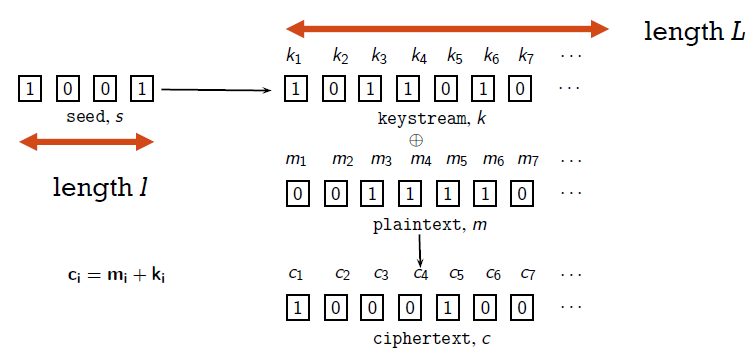
\includegraphics[width=0.7\linewidth]{Images/Chapter2/screenshot000}
	\caption{}
	\label{fig:chapter2_screenshot000}
\end{figure}


For a stream cipher to be good, Eve should not be able to: recover the seed by making the set of possible seeds so large that and exhaustive search is very hard in practice and also predict the rest of the keystream by eliminating any patterns from the keystream.
More precisely: choose a short $l$-bit (much smaller than the lenght L of the plaintext to be encrypted) seed $s$ as the encryption key and stretch the seed into a longer $L$-bit string (the key) that is used  to mask the message and decrypt the ciphertext. The seed $s$ is stretched using some efficient, deterministic algorithm G that maps $l$-bit strings (seeds) to $L$-bit strings(keys). Formally:
\begin{itemize}
	\item Encryption: $G(s)+m$ for any seed s (of size l) and plaintext m (of size L)
	\item Encryption: $G(s) + c$ for any seed s (of size l) and ciphertext c (of size L) where $G$ is called a pseudo-random generator
\end{itemize}

Notice that if $l<L$, then by Shannon’s Theorem, stream ciphers cannot be perfect, however, if G has certain properties, then stream ciphers are secure in practice. Suppose $s$ is a random $l$-bit string and $r$ is a random $L$-bit string, if Eve cannot effectively tell the difference between $G(s)$ and $r$, then it should not be able to tell the difference between stream ciphers and one-time pad. Since the one-time pad latter cipher is secure, so should be the stream cipher.

A stream-cipher is well equipped to encrypt a single message from Alice to Bob. If two messages are encrypted with the same key there may be problems. As an example consider the case in which Alice and Bob want to exchange messages $m_1$ and $m_2$, let $c_1 = m_1 + G(s)$ and $c_2 = m_2 + G(s)$. If Eve is able to intercept both ciphertexts, then it is able to calculate $c_1 + c_2 = ( m_1 + G(s)) + (m_2 + G(s)) = (m_1 + m_2) + (G(s) + G(s)) = m_1 + m_2$, and as english text contains enough redundancy that given $m_1 + m_2$, Eve can recover both m1 and m2 in the clear by using frequency analysis.

Stream-ciphers are said to be malleable since an attacker can cause predictable changes to the plaintext, this is because and attacker can intercept ciphertext $c$ and forwarding $c^'=c+d$, effectively the receiver will get $m' = c' + G(s)= (c+d) + G(s) = (c+G(s)) + d = m + d$. In other words knowing neither $m$ nor $s$, Eve was able to cause the decrypted message to become $m + d $ for $d$ of its choice.

In summary stream-ciphers do not give rise to error propagation as each bit in the ciphertext depends on just one bit in the plaintext and 1 bit transmission errors will result in 1 bit error in the plaintext, also they are very fast making them ideal for real time applications (e.g., mobile communication services) and easy to implement in hardware and don't require large memory capabilities. Since stream ciphers process data bitwise, it is crucial that sender and receiver keep their keystreams in perfect synchronization and 1 bit data loss may have catastrophic consequences as decryptions are performed on the wrong bits after the receiver is out of sync of the sender and re-synchronization mechanisms must be put in place to avoid these problems.


\subsection{Vigenère cipher}

It can be seen as a variant of Vernam cipher whereby the key is a sequence of bits of fixed length. The key, and plaintext are a string of bytes, to encrypt: XOR each character in the plaintext with the next character of the key and wrap around in the key as needed.

Vigenere cipher can be attacked by first determining the key length and determining each byte of the key by using frequency analysis.

\subsection{Block ciphers}

Replace a block of N bits from the plaintext with a block of N bits from the ciphertext. 
\begin{figure}
	\centering
	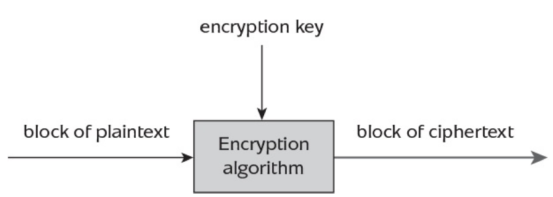
\includegraphics[width=0.7\linewidth]{Images/Chapter2/screenshot001}
	\caption{}
	\label{fig:chapter2_screenshot001}
\end{figure}

\begin{figure}
	\centering
	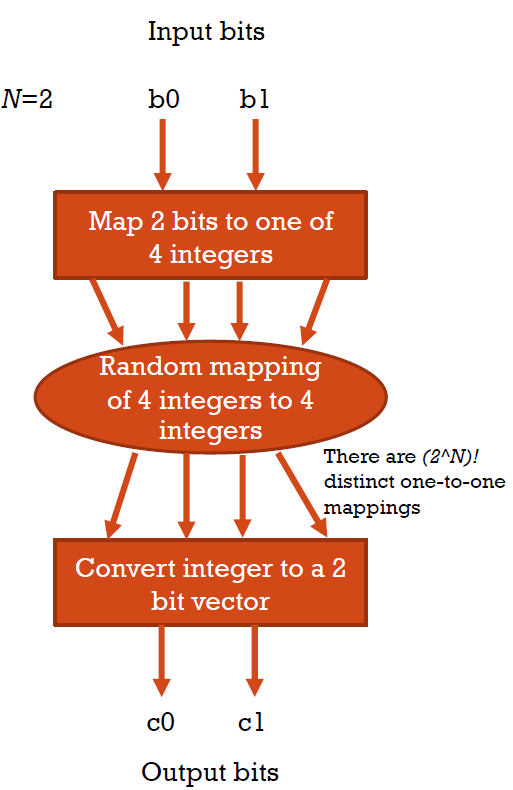
\includegraphics[width=0.4\linewidth]{Images/Chapter2/screenshot002}
	\caption{}
	\label{fig:chapter2_screenshot002}
\end{figure}

The relationship between the input blocks and the output block is completely random. It must be invertible for decryption to work. Thus, it has to be one-to-one, i.e. each input block is mapped to a unique output block. Usually, N=64, 128, 256. If the block size is too small, then the number of different plaintext blocks that can ever be encrypted may be too small for an attacker to launch a type of dictionary attack by building up a dictionary of plaintext/ciphertext pairs, if the block size is too large, then the block cipher becomes inefficient to operate, particularly for plaintexts smaller than the block size as they need padding. The encryption key for the ideal block cipher is the table (also called the codebook) that shows the relationship between the input and the output blocks. Think of each possible input block as one of $2^N$ integers and for each such integer we can specify an output $N$-bit block. If $N$ is 64 then the codebook will be of size $N*(2^N)$ which is around $10^(21)$, but this is not practical since we can can not share such keys.

To make this practical a block cipher is a keyed family of pseudorandom permutations For each key, we have a single permutation that is independent of all the others. Think of each key as corresponding to a different codebook and our strategy is to choose $2^K$ permutations uniformly at random from the set of all $(2^N)!$ permutations

Block ciphers are slower than stream ciphers but are generally considered more secure than the latter.
Block ciphers have a property called diffusion: 2 blocks differing in a single bit shall generate 2 very different ciphertexts. So even a small transmission error will give rise to errors in around half of the bits in the plaintext.


\section{Examples of symmetric ciphers}

\begin{figure}
	\centering
	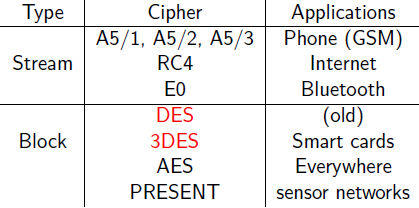
\includegraphics[width=0.7\linewidth]{Images/Chapter2/screenshot003}
	\caption{}
	\label{fig:chapter2_screenshot003}
\end{figure}

\subsection{Examples of stream ciphers}
\begin{itemize}
	\item RC4: Simple and fast stream cipher with a relatively low level of security, probably the most widely implemented stream cipher in software and widely used in SSL/TLS, WEP, and Microsoft Office
	\item A5/1: One of the stream cipher algorithms used in GSM to secure the communication channel over the air from a mobile phone to the nearest base station
	\item E0: The stream cipher algorithm used to encrypt Bluetooth communications
\end{itemize}

\subsection{Examples of block ciphers}

\begin{itemize}
	\item DES: The default block cipher of the 1980s and 1990s, but now considered broken due primarily to its small key size. The two variants based on repeated DES applications commonly known as 3DES are still respected block ciphers, although there are now faster block ciphers available.
	\item AES: A default block cipher based on the encryption algorithm Rijndael which won the AES design competition by NIST to identity the successor of DES
	\item Serpent: A respected block cipher with a block size of 128 bits and key lengths of 128, 192, or 256, which was a finalist with AES in the NIST competition. Considered slower but somehow more secure than AES but not as widely adopted
\end{itemize}

\section{Implementation of stream ciphers}

First we want to tackle the problem of generating a randomly a key (known as keystream )that is as long as possible. Keystream generators should be fast (as in computable in polynomial time as function of number $l$ of bits in the seed) and be secure, so intuitively, a string of L bits produced by a keystream generator should look random. I.e. it should be impossible in a polynomial amount of time in l to distinguish between a truly random bit string of length L and a string of the same length returned by the keystream generator. The main components are:
\begin{itemize}
	\item States: vector of bits organized in registers
	\item Update function: function mapping a state to the next state (clock function)
	\item Output function: function extracting a bit from a state. Concatenating all bits returned by this function, it is possible to obtain the keystream
	\item Key loading: function that takes the seed (secret) and a (public) Initialization Vector (IV) to compute the initial state for the update function. Each IV should be used only once.
\end{itemize}

\begin{figure}
	\centering
	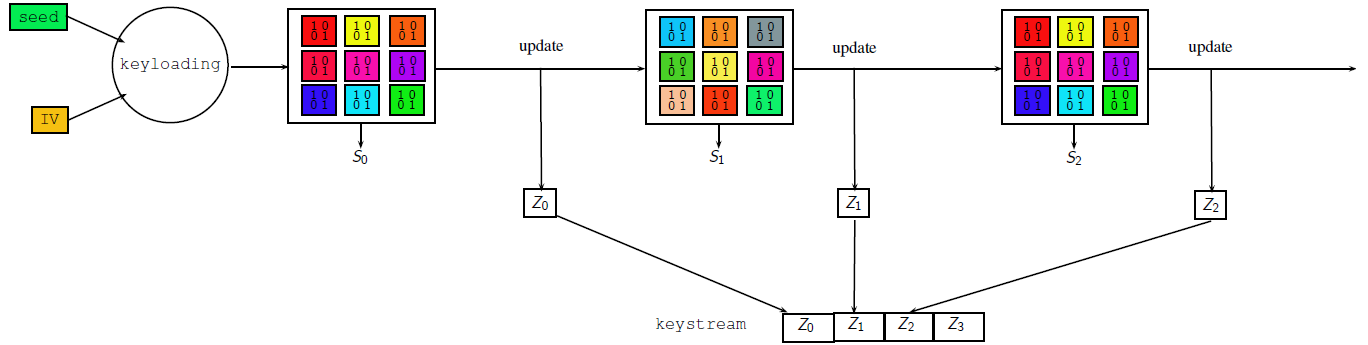
\includegraphics[width=0.9\linewidth]{Images/Chapter2/screenshot004}
	\caption{}
	\label{fig:chapter2_screenshot004}
\end{figure}

\section{Warm Up}

The first output bits strongly depend on the initial state. To avoid potential problems, it is customary to run a warm-up phase before starting encryption. This preliminary phase consists in applying the update function several times without outputting any bits of keystream and it is a highly recommended security best practice.
Given any initial state, the states are periodic, since they are in a finite number and at some point we will obtain again one of the previous states. The keystream is also periodic... this is impossible to avoid. The smallest number $i$ such that $update(...(update(S)))=S$ is called the period of the keystream (it depends on the initial state), and as a requirement is that the period of the keystream shall be quite large, regardless of the initial state, and can be achieved by a suitable design of the update function.
As an example let's take an un update function as follows $f: (x,y,z) \Rightarrow (y+z,x,y)$. One can see that the repeated application of $f$ to the inital state $(1,0,1)$ will yield $(1,0,1) \Rightarrow (1,1,0) \Rightarrow (1,1,1) \Rightarrow (0,1,1) \Rightarrow (0,0,1) \Rightarrow (1,0,0) \Rightarrow (0,1,0) \Rightarrow (1,0,1)$ with a period of 7.
We are using linear functions because they are easy to implement and compute.

\section{Linear feedback shift register}

A linear feedback shift register of length n is a shift register composed by n bits.
Type of digital circuit using a cascade of flip flops where the output of one flip-flop is connected to the input of the next.
Flip-flops share a single clock signal, which causes the data stored in the system to shift from one location to the next.

Now we add the linear feedback function.

A linear-feedback shift register (LFSR) is a shift register whose input bit is a linear function of its previous state. Essentialy feed the output of flip flops to the linear function.

The most commonly used linear function of single
bits is xor. An LFSR is usually a shift register whose input bit is driven by the xor of some bits of the overall
shift register value. The initial value of the LFSR is called the seed. Since the operation of the register is deterministic, the stream of values produced by the register is completely determined by its current (or previous) state.

Return the output of the linear function as input to the first flip flop.


\section{LSR and finite fields}

Longest possible cycle.
We have a finite set of states, and an uodate function, we want a function that genertes all possible elements in the set, and repeats as late as possible.


The algebraic stucture we are using is multiplication modulo a prime.
What we need are polynomial over a Galois field.
If you multiply a polinomial with a monomial is "equal" to the shift right operation.

Mathemaricians provided a table for each number of bits and a polynomial to generate all possibile polynomials.

Important: these functions are guaranteed to generate the longes possibile sequence with a fixed number of bits.


Take the number of flipflops that we need, put a linear feedback function that is a linear combination of the registers. For 4 registers we have x^4 + x^3 + 1 and taps are 1100. So we consider only the output of the first two registers to the left. So first we perform and AND operation with 1100 and finally a xor operation and we are guaranteed to generate the longest sequence. But is this a good idea? 

No, attacks to this are very easy. We'll use 128 bits but as of now we offer very low protection.

Exploit the connection with linear algebra.
Collect enough bits and then by solving a bunch of equations recover the seed. So recover the seed in polynomial time.

Linearity is good because it is easy to implement, but on the other hand is not secure enough.


Consider two linear shift register, and run them in parallel and combine the result of the two with a non linear operation. The 40 bit seed is distributed to the two registers.



\section{A5 Family of Ciphers}

GSM = Global System for Mobile communication (ETSI standard).

We generate a new session every time? Because if the attacker breaks one session, he breaks every other session.


An algorithm of the A5 family takes § the session key Kc (symmetric) and a frame counter Fn generates § 228 pseudo random bits (PRAND), called a key stream.
The key stream is then XORed with a 228 bit segment of plain text, yielding 228 bits of ciphertext.

Members of the A5 family differs on how GEN is implemented, thereby providing different levels of security.


A5/2 after a month an attack was found that could break the cipher almost in real time.

A5/3 is the last stream cipher of the A5 family and provides users with a higher level of security than both A5/1 and A5/2. It is based on the block cipher KASUMI. 


\section{Remarks on the A5 Family}

The generated key (Kc) is the main flaw of the design:
\begin{itemize}
	\item Maximal exhaustive search complexity is (only) $2^(64)$
	\item  Kc generated only once after the cell phone registers with the network and stays active for all communication, until the telco requests a new one or the cell phone deregisters 
	\item Kc is artificially shortened in deployed systems when zeroing 10 bits, lowering search complexity to $2^(54)$
	\item Encryption is applied after error correction
	\item A5/2 is extremely weak and it can be broken in real time with inexpensive equipment; it is therefore no longer supported by new mobile phones
	\item A5/1 is affected by a number of serious weaknesses, and its use is strongly discouraged, since there are practical attacks that can break the cipher
	\item  A5/3 is the common standard for the new generation of mobile and it is considered secure, even though there do exist practical attacks to KASUMI that suggest some significant weaknesses of the cipher
\end{itemize}

\section{Practicality of attacking GSM communication}

In theory, the attacks are relatively simple
In practice, a considerable amount of hardware is necessary to actually intercept GSM communications
The hardware must at least consist of a radio receiver device which is capable of receiving and decoding digital data that is exchanged over-the-air by using one of the attacks reported above
Hypothetically a simple GSM mobile phone already has all these capabilities (except the decrypting of an unknown A5 stream), so it might be possible to use such a phone for eavesdropping
Nevertheless a huge amount of know-how, time and money is needed

\section{Bluetooth}
Bluetooth is a wireless technology standard invented by Ericsson in 1994 for exchanging data over short distances using short-wavelength UHF radio waves (Range: 2.4 to 2.485 GHz) from fixed and mobile devices.
The standard offers methods for generating keys, authenticating users, and encrypting data.


Stream ciphers transform the problem to generating a long stream of bytes that looks like random but it reproducible with a given seed. The strength of stream ciphers comes from how good it can approximate randomness. We used LSFR because they are really cheap and it is easy to implement the shift and generate long streams of seemingly random data. The important property is that they should generate the longest possible sequence before repeating them selves, and that is $2^n$. We exploit the connection with Galois field. The coefficients of the polynomial correspond with the taps of the LFSR. LFSR are easy to invert so we need to do something better.

\section{RC4}

Invented by Rivest, the inventor of RSA! It was secret, but then someone reverse engineered it. Used a lot, operates on bytes, it is simple and fast.

The basic data structure needed is an array of 256 bytes, called the state vector $S$ containing values from 0 to 255 in an increasing order. Then you start scrambling these bytes by using a key $T$. The key if shorter is repeated.

But why use $j = (j + S[i] + T[i]) mod 256$? Because it works in practice. It is also easy to compute.
The way you pick indexes is biased.

RC4 in WEP. But is vulnerable!
Now we use WPA2, is not perfect, it used AES.

We need to derive a session key starting from a pre shared key. So that the session key is unique between devices.

TKIP implements a key mixing function that combines the pre shared key with....

We avoid using a key using more than once. 

\begin{figure}
	\centering
	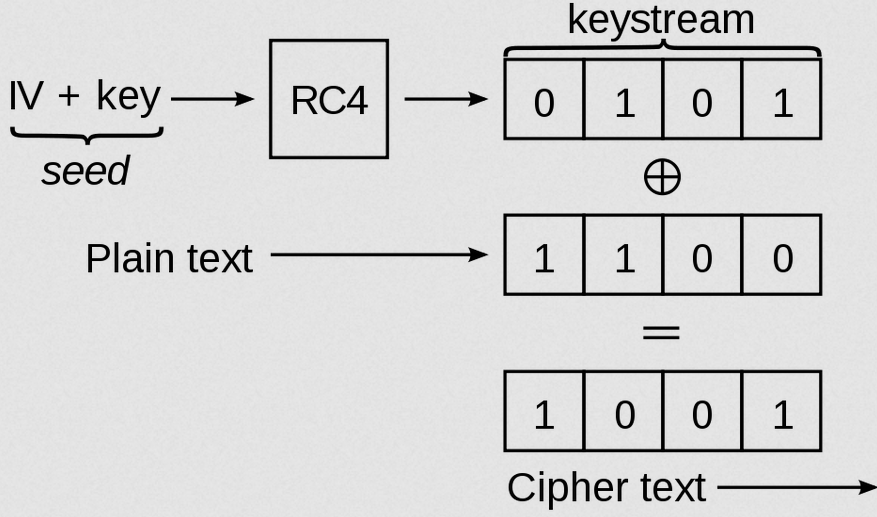
\includegraphics[width=0.7\linewidth]{Images/Chapter2/screenshot014}
	\caption{}
	\label{fig:chapter2_screenshot014}
\end{figure}

Security of WPA2.

Vulnerable to KRACK attack. It exploits a functionality where if a user is disconnected from wifi then for reconnecting it performs an easier problem to derive a new session.

We should use different ciphers for different context. 